%----------------------------------------------------------
\def\notedate{2021.11.14}
\def\currentauthor{Муха В. (РК6-73Б)}
%----------------------------------------------------------
\notestatement{rndhpcedt}{Первичный обзор литературы}

%----------------------------------------------------------
\subsubsection{Известные алгоритмы поиска циклов в графах}

Существует несколько групп алгоритмов поиска\cite{davidrajuh2016}:
\begin{enumerate}[label=\arabic*)]
    \item алгоритмы поиска ориентированных графов;
    \item алгоритмы, основанные на использовании матриц смежности
\end{enumerate}

Одним из представителей алгоритмов поиска является алгоритм поиска в глубину depth-first-search (DFS). Сложность алгоритма $O(n^2)$ для обхода из одного узла и $O(n^3)$ - общая сложность обхода из всех узлов. Поэтому для ускорения алгоритма необходимо применение модификаций, например распараллеливание алгоритма поиска в глубину.\cite{Mahdi2011}.

Зададим граф $G(V, E)$, где $V$ -- это множество вержин графа $(a, g)$, а $E$ -- это множество рёбер графа $(ab, ad, ... , ge)$. Сам граф $G$ и его матрица смежности $A$ приведены ниже.

\begin{figure}[H]
	\centering
	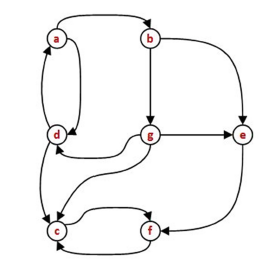
\includegraphics[width=0.3\textwidth]{ResearchNotes/rndhpc_not_edt_2021_11_14/adj_matrix.png}
	\caption{Граф и его матрица смежности} 
\end{figure}

Матрица смежности $A$ показывает исходящие соединения вершин из узла, а транспонированная матрица $A^T$ показывает входящие соединения в узел. Степень матрицы $A^n$ - это число соединений узлов состоящих ровно из $n$ узлов.
Для того, чтобы определить циклы порядка $2n$, нужно найти матрицу циклов $C^n$. Её можно найти, применив операцию \textsf{AND} над матрицами $A^n$ и $(A^n)^T$ для каждого элемента матриц.

\begin{equation}
    C^n = (A^n \wedge (A^n)^T)
\end{equation}

Таким образом, матрица $C^n$ будет содержать все циклы порядка $2n$. Для поиска циклов порядка $[2, 2n]$ необходимо повторить операцию $n$ раз.

%----------------------------------------------------------
\subsubsection{Пересчет циклов в графах в т.ч. при помощи GPU}

\begin{remark}
Пересчет циклов в графе является NP-полной задачей\cite{Mahdi2011}, следовательно не может быть выполнен за полиномиальное время.
\end{remark}

В статье \cite{Mahdi2011} представлен подход, позволяющий ускорить процедуру пересчета циклов с использованием \textsf{GPU}, описываемый алгоритмом \ref{algo.cycles.search}.

\begin{algorithm}[H]
\caption{Алгоритм Thread-Based Cycle Detection поиска циклов в ориентированном графе}\label{algo.cycles.search}
\begin{algorithmic}[1]
	\State Создаем массив узлов графа $V$.
	\State Заполняем новый массив $V'$ вершинами со степенью больше чем 2 -- это исключит узлы, которые не могут иметь цикла. 
	\State Для каждого элемента массива $V$ параллельно создаём комбинацию для проверки.
	\State Создаём матрицу смежности $C$ для созданной комбинации и проверяем её на наличие циклов.
	\State Меняем комбинации перестановками.
\end{algorithmic}
\end{algorithm}

%----------------------------------------------------------
% Атрибуты задачи
\noteattributes{}
%----------------------------------------------------------